\subsection{Специальный фильтр}

Будем рассматривать линейный фильтр второго порядка вида: 
\begin{equation}
    W_2(p) = \frac{(T_1p + 1)^2}{(T_2p + 1)(T_3p + 1)} = \frac{T_1^2p^2 + 2T_1p + 1}{T_2T_3p^2 + (T_2 + T_3)p + 1}
\end{equation}

Для того, чтобы подобрать коэффициенты $T_1$, $T_2$, $T_3$, я рассмотрел данный фильтр в виде произведения двух фильтров первого порядка. 
В ходе рассмотрения графиков АЧХ данных фильтров я пришел к выводу, что, можно ввести параметры $w_0$ и $A$ -- частота, на которой происходить фильтрация и коэффициент подавления на этой частоте соответственно.
коэффициенты исходного фильтра получаются следующим образом:
\begin{equation}
    T_1 = \frac{1}{w_0}, \quad T_2 = \frac{A}{w_0}, \quad T_3 = \frac{1}{Aw_0}
    \label{eq:t_params}
\end{equation}

\def\num{6}
\def\a{4}
\def\from{1}
\def\to{4}
\def\b{0}
\def\c{0.4}
\def\d{80}
\def\L{10}
\def\A{30}
\def\Wz{80}
\def\Tf{\fpeval{round(1 / \Wz, 7)}}
\def\Ts{\fpeval{round(\A / \Wz, 7)}}
\def\Tt{\fpeval{round(1 / (\A * \Wz), 7)}}

\subsubsection{Рассматриваемая функция}
Рассмотрим функцию $g(t)$ при параметрах $a=\a$, $t_1 = \from$, $t_2 = \to$ ~(см. рисунок~\ref{fig:wave_func_\num}) 
и ее \textit{зашумленную} версию $u(t)$ с параметрами $b = \b$, $c = \c$, $d = \d$ ~(см. рисунок~\ref{fig:noised_wave_func_\num}).
на промежутке $[0,\L]$. 

\subsubsection{Графики рассматриваемой и зашумленной функции}
\begin{figure}[ht!]
    \centering
    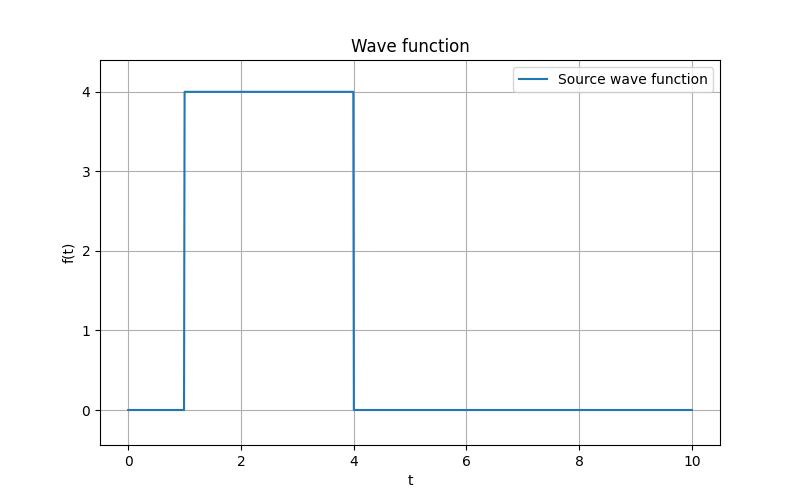
\includegraphics[width=\textwidth]{../results/second/\num/wave_func.png}
    \caption{Функция $g(t)$ с параметрами $a = \a$, $t_1 = \from$, $t_2 = \to$}
    \label{fig:wave_func_\num}
\end{figure}

\begin{figure}[ht!]
    \centering
    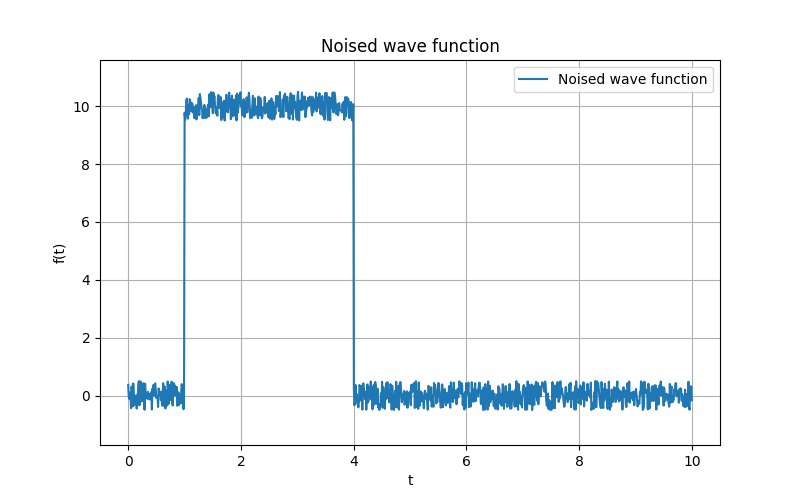
\includegraphics[width=\textwidth]{../results/second/\num/noised_wave_func.png}
    \caption{Функция $u(t)$ с параметрами $b = \b$, $c = \c$, $d = \d$}
    \label{fig:noised_wave_func_\num}
\end{figure}

\FloatBarrier
\subsubsection{Применение фильтра}

Рассмотрим фильтрованную функцию $u'(t)$, которая получается применением линейного фильтра второго порядка с $T_1 = \Tf$, $T_2 = \Ts$, $T_3 = \Tt$ (см. рисунок \ref{fig:noised_wave_func_filtered_\num}).
Значения $T_1,~T_2,~T_3$ получены из формул \eqref{eq:t_params} при $w_0 = \Wz$ и $A = \A$.

\begin{figure}[ht!]
    \centering
    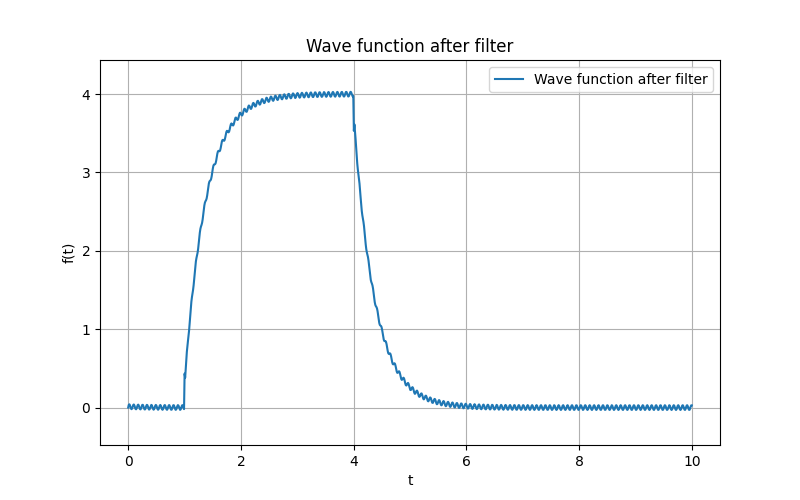
\includegraphics[width=\textwidth]{../results/second/\num/noised_wave_func_filtered.png}
    \caption{Функция $u'(t)$ после применения фильтра}
    \label{fig:noised_wave_func_filtered_\num}
\end{figure}

Видим, что функция после фильтрации стала более гладкой, фронт и спад стали менее выраженными.
Это связано с тем, что фильтр убирает высокочастотные компоненты функции. Убедиться в этом можно 
посмотрев на АЧХ фильтра (см. рисунок \ref{fig:filter_frequency_response_\num} и \ref{fig:filter_frequency_response_log_\num}).

\FloatBarrier
\subsubsection{Амплитудно-частотная характеристика фильтра}
\begin{figure}[ht!]
    \centering
    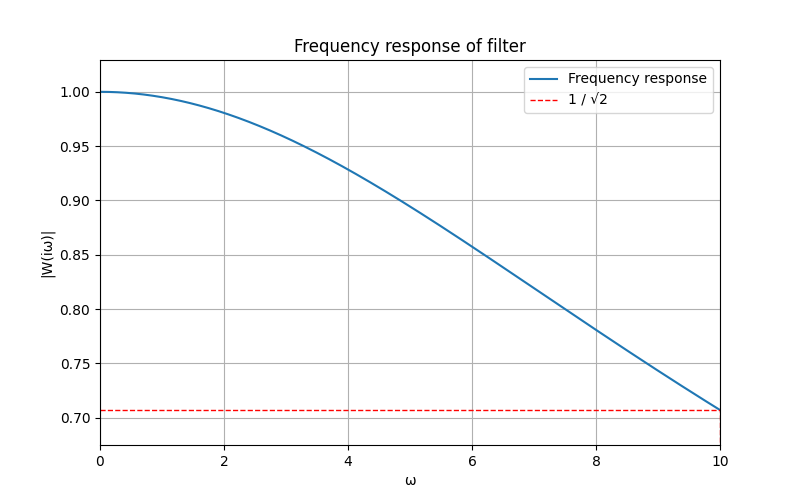
\includegraphics[width=\textwidth]{../results/second/\num/filter_frequency_response.png}
    \caption{АЧХ фильтра второго порядка при $T_1 = \Tf$, $T_2 = \Ts$, $T_3 = \Tt$}
    \label{fig:filter_frequency_response_\num}
\end{figure}

\begin{figure}[ht!]
    \centering
    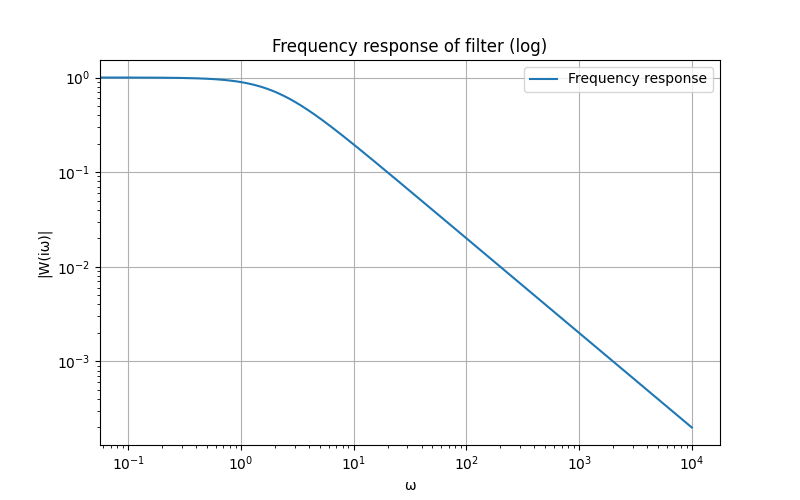
\includegraphics[width=\textwidth]{../results/second/\num/filter_frequency_response_log.png}
    \caption{АЧХ фильтра второго порядка при $T_1 = \Tf$, $T_2 = \Ts$, $T_3 = \Tt$ (логарифмическая шкала)}
    \label{fig:filter_frequency_response_log_\num}
\end{figure}

На логарифмическом графике более заметно, что данный фильтр подавляет частоты в окрестности частоты $w_0 = \Wz$, что и требуется для фильтрации гармонического шума. 
Но, на этом же графике видно, что фильтр, кроме требуемых частот, подавляет довольно большой диапазон частот, что, конечно, сильно сказывается на качестве фильтрации. 
Именно для того, чтобы фильтр минимально срезал нижние частоты, которые необходимы для восстановления исходной функции была выбрана довольно большая частота гармонического шума.

\FloatBarrier
\subsubsection{Результаты фильтрации}
Сравнительный график исходной функции и функции после фильтрации представлен на рисунке \ref{fig:wave_func_cmp_\num}.

\begin{figure}[ht!]
    \centering
    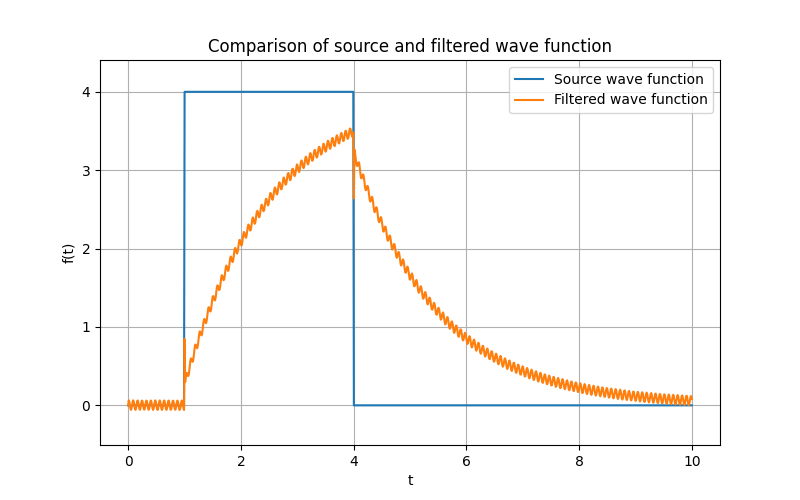
\includegraphics[width=\textwidth]{../results/second/\num/wave_func_cmp.png}
    \caption{Сравнение функции $g(t)$ и $u'(t)$}
    \label{fig:wave_func_cmp_\num}
\end{figure}

Образ исходной функции и функции после фильтрации приведены на рисунках \ref{fig:wave_func_image_\num}~и~\ref{fig:noised_wave_func_filtered_image_\num}.
Графики модулей соответствующих функций приведены на рисунках~\ref{fig:wave_func_image_abs_\num}~и~\ref{fig:noised_wave_func_filtered_image_abs_\num}, их 
сравнительный график -- на рисунке~\ref{fig:wave_func_image_cmp_\num}.

На сравнительном графике (см. рисунок~\ref{fig:wave_func_image_cmp_\num}) видно, что \textit{амплитуда} образа фильтрованного сигнала уменьшается по сравнению 
с образом начальной функции. Результат соответствует АЧХ фильтра (см. рисунок~\ref{fig:filter_frequency_response_\num}).

\begin{figure}[ht!]
    \centering
    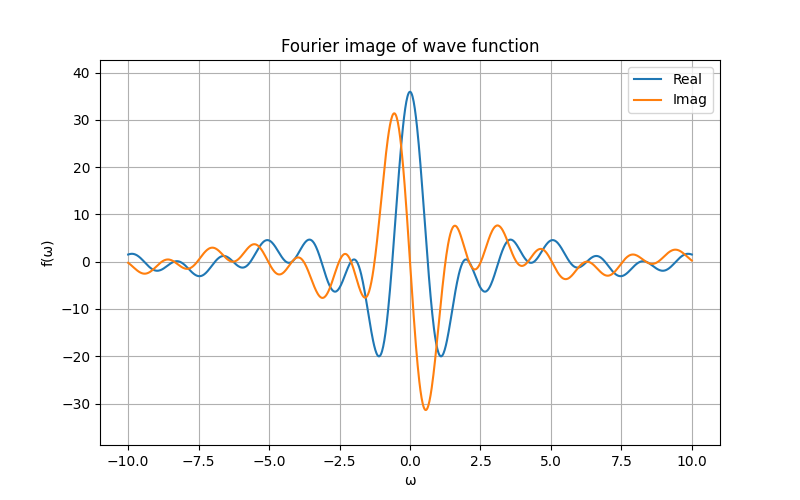
\includegraphics[width=\textwidth]{../results/second/\num/wave_func_image.png}
    \caption{Образ исходной функции $u(t)$.}
    \label{fig:wave_func_image_\num}
\end{figure}

\begin{figure}[ht!]
    \centering
    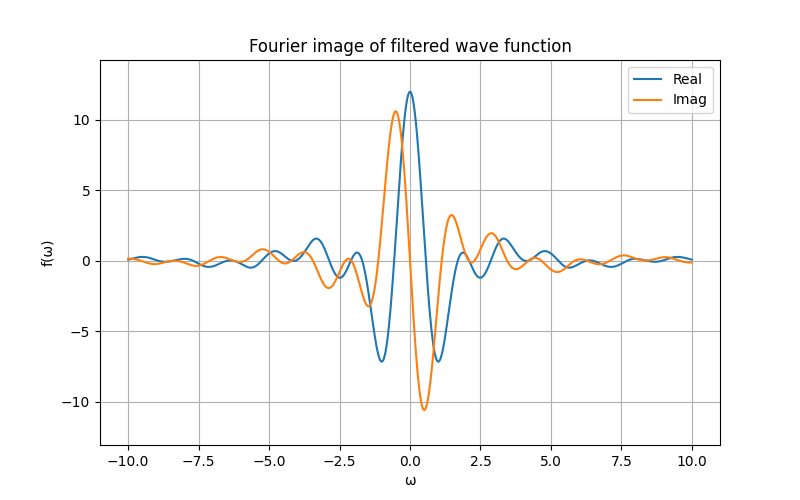
\includegraphics[width=\textwidth]{../results/second/\num/noised_wave_func_filtered_image.png}
    \caption{Образ фильтрованной функции $u'(t)$.}
    \label{fig:noised_wave_func_filtered_image_\num}
\end{figure}

\begin{figure}[ht!]
    \centering
    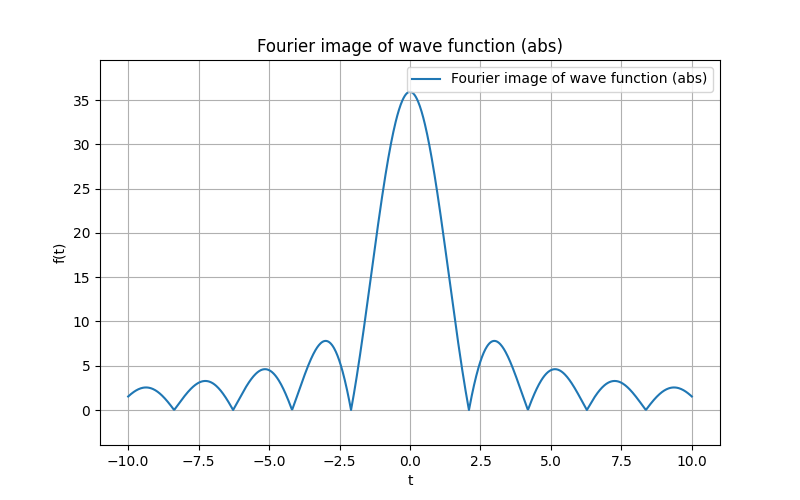
\includegraphics[width=\textwidth]{../results/second/\num/wave_func_image_abs.png}
    \caption{Модуль образа исходной функции $u(t)$.}
    \label{fig:wave_func_image_abs_\num}
\end{figure}

\begin{figure}[ht!]
    \centering
    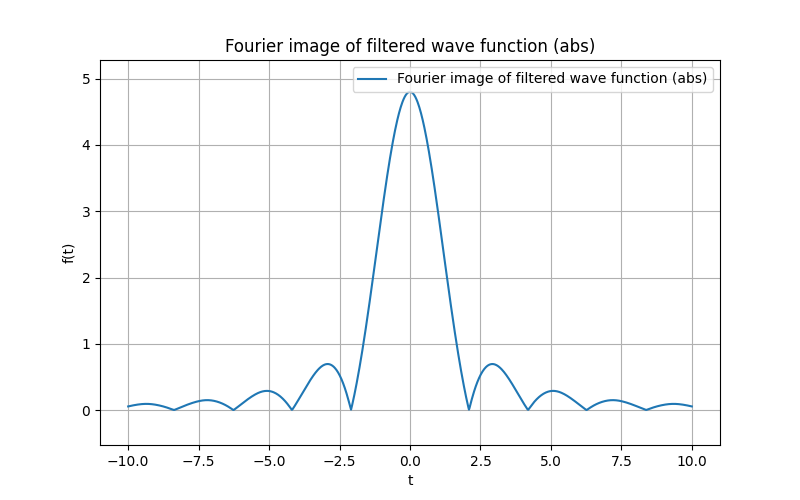
\includegraphics[width=\textwidth]{../results/second/\num/noised_wave_func_filtered_image_abs.png}
    \caption{Модуль образа фильтрованной функции $u'(t)$.}
    \label{fig:noised_wave_func_filtered_image_abs_\num}
\end{figure}

\begin{figure}[ht!]
    \centering
    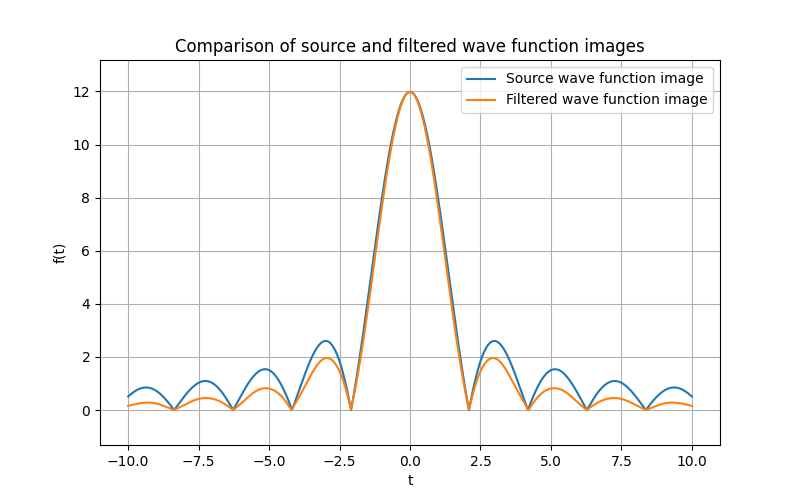
\includegraphics[width=\textwidth]{../results/second/\num/wave_func_image_cmp.png}
    \caption{Сравнение модулей образов исходной и фильтрованной функций.}
    \label{fig:wave_func_image_cmp_\num}
\end{figure}

\FloatBarrier
\subsubsection{Фильтрация шума меньшей частоты}

\def\num{7}
\def\a{4}
\def\from{1}
\def\to{4}
\def\b{0}
\def\c{0.4}
\def\d{20}
\def\L{10}
\def\A{30}
\def\Wz{20}
\def\Tf{\fpeval{round(1 / \Wz, 7)}}
\def\Ts{\fpeval{round(\A / \Wz, 7)}}
\def\Tt{\fpeval{round(1 / (\A * \Wz), 7)}}

Теперь рассмотрим функцию с гармоническом шумом меньшей частоты, чем в предыдущем случае: 
$g(t)$ при параметрах $a=\a$, $t_1 = \from$, $t_2 = \to$ ~(см. рисунок~\ref{fig:wave_func_\num}) 
и ее \textit{зашумленную} версию $u(t)$ с параметрами $b = \b$, $c = \c$, $d = \d$ ~(см. рисунок~\ref{fig:noised_wave_func_\num}).
на промежутке $[0,\L]$. 

\begin{figure}[ht!]
    \centering
    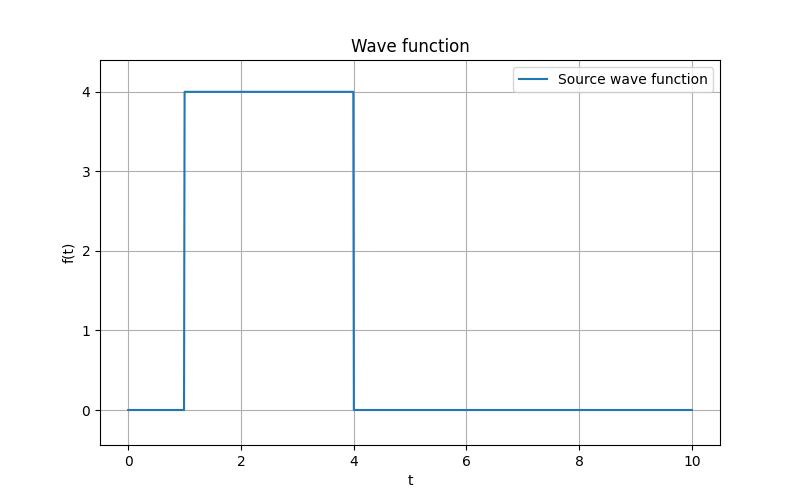
\includegraphics[width=\textwidth]{../results/second/\num/wave_func.png}
    \caption{Функция $g(t)$ с параметрами $a = \a$, $t_1 = \from$, $t_2 = \to$}
    \label{fig:wave_func_\num}
\end{figure}

\begin{figure}[ht!]
    \centering
    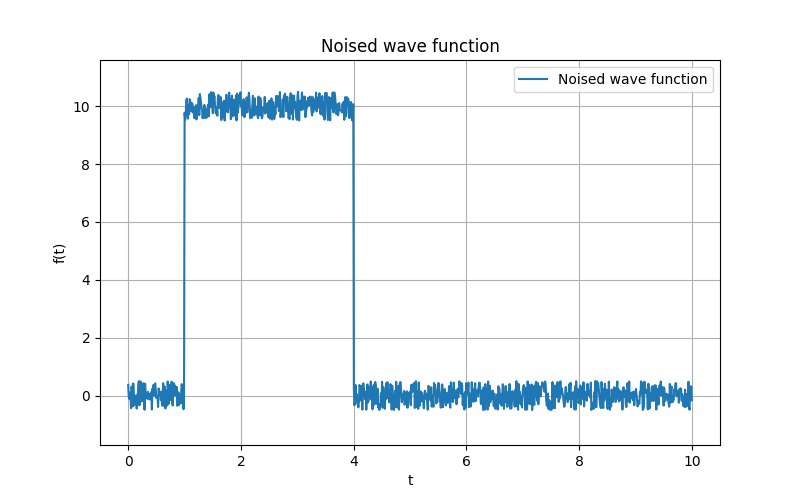
\includegraphics[width=\textwidth]{../results/second/\num/noised_wave_func.png}
    \caption{Функция $u(t)$ с параметрами $b = \b$, $c = \c$, $d = \d$}
    \label{fig:noised_wave_func_\num}
\end{figure}

Рассмотрим фильтрованную функцию $u'(t)$, которая получается применением линейного фильтра второго порядка с $T_1 = \Tf$, $T_2 = \Ts$, $T_3 = \Tt$ (см. рисунок \ref{fig:noised_wave_func_filtered_\num}).
Значения $T_1,~T_2,~T_3$ получены из формул \eqref{eq:t_params} при $w_0 = \Wz$ и $A = \A$.

\begin{figure}[ht!]
    \centering
    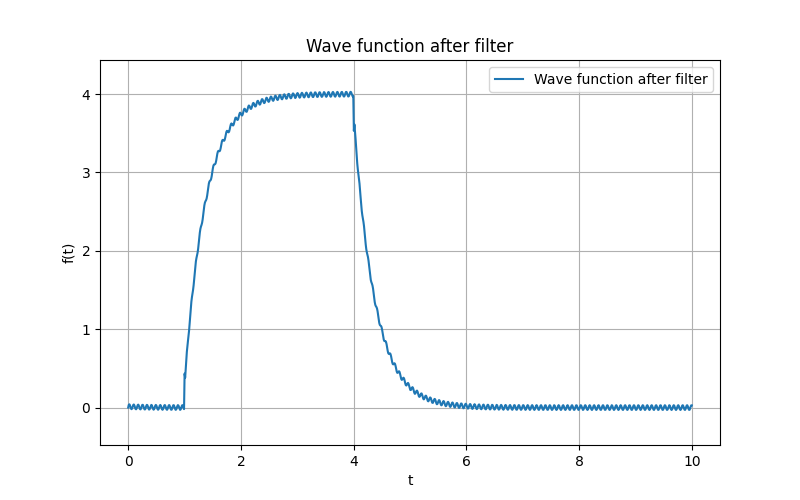
\includegraphics[width=\textwidth]{../results/second/\num/noised_wave_func_filtered.png}
    \caption{Функция $u'(t)$ после применения фильтра}
    \label{fig:noised_wave_func_filtered_\num}
\end{figure}

На рисунке~\ref{fig:noised_wave_func_filtered_\num} видно, что гармонический шум действительно уменьшился, при этом,
фронт и спад функции стали менее выраженными. Это связано с тем, что фильтр убирает не только частоты гармонического шума,
но и некоторый диапазон частот рядом с ним, что и приводит к сглаживанию функции.
Убедить в этом можно посмотрев на графики АЧХ данного фильтра (см. рисунок \ref{fig:filter_frequency_response_\num} и \ref{fig:filter_frequency_response_log_\num}).

\begin{figure}[ht!]
    \centering
    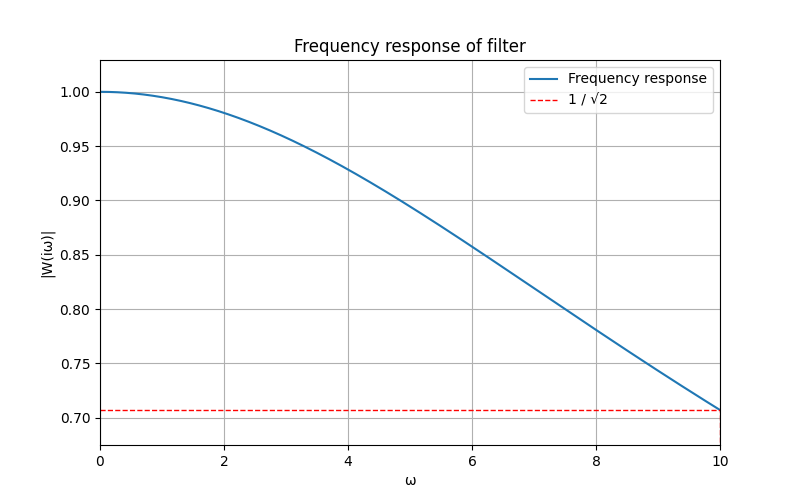
\includegraphics[width=\textwidth]{../results/second/\num/filter_frequency_response.png}
    \caption{АЧХ фильтра второго порядка при $T_1 = \Tf$, $T_2 = \Ts$, $T_3 = \Tt$}
    \label{fig:filter_frequency_response_\num}
\end{figure}

\begin{figure}[ht!]
    \centering
    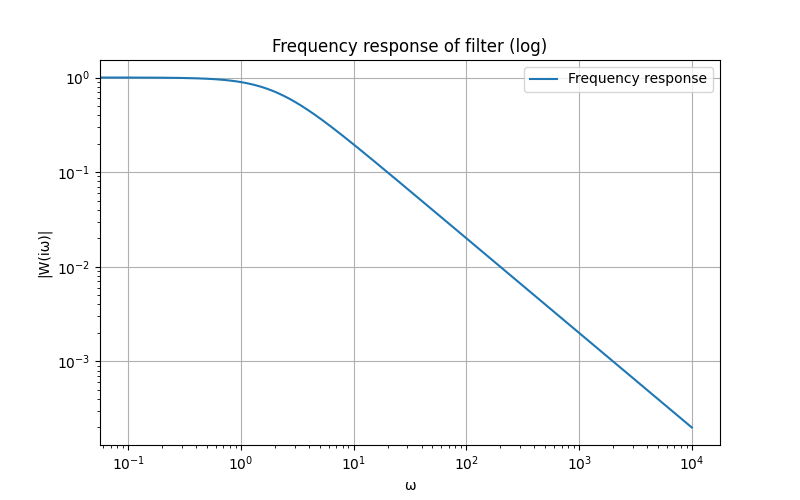
\includegraphics[width=\textwidth]{../results/second/\num/filter_frequency_response_log.png}
    \caption{АЧХ фильтра второго порядка при $T_1 = \Tf$, $T_2 = \Ts$, $T_3 = \Tt$ (логарифмическая шкала)}
    \label{fig:filter_frequency_response_log_\num}
\end{figure}

Сравнительный график исходной и фильтрованной функции приведен на рисунке~\ref{fig:wave_func_cmp_\num}.
\begin{figure}[ht!]
    \centering
    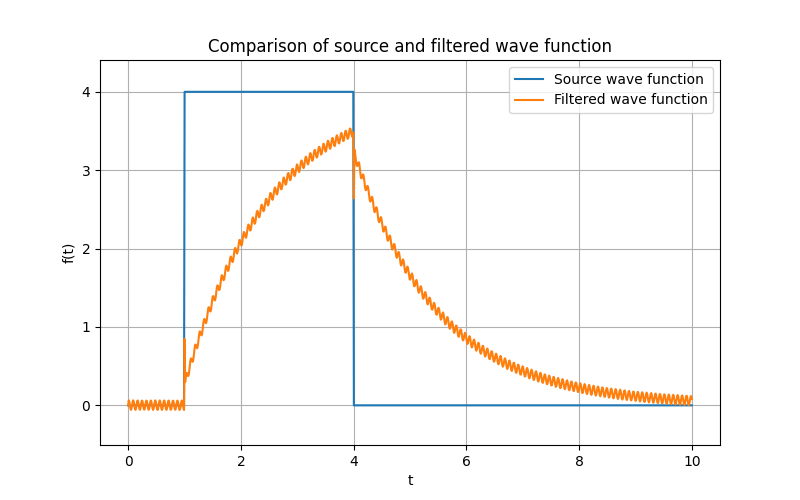
\includegraphics[width=\textwidth]{../results/second/\num/wave_func_cmp.png}
    \caption{Сравнение функции $g(t)$ и $u'(t)$}
    \label{fig:wave_func_cmp_\num}
\end{figure}

\FloatBarrier
\subsubsection{Фильтрация шума большей частоты}

\def\num{8}
\def\a{4}
\def\from{1}
\def\to{4}
\def\b{0}
\def\c{1}
\def\d{2000}
\def\L{10}
\def\A{300}
\def\Wz{2000}
\def\Tf{\fpeval{round(1 / \Wz, 7)}}
\def\Ts{\fpeval{round(\A / \Wz, 7)}}
\def\Tt{\fpeval{round(1 / (\A * \Wz), 7)}}

Теперь рассмотрим более удачный случай, когда гармонический шум имеет большую частоту. Такую, что
при применении фильтра не будет захватываться диапазон частот, необходимый для восстановления исходной функции.

Рассмотрим функцию $g(t)$ при параметрах $a=\a$, $t_1 = \from$, $t_2 = \to$ ~(см. рисунок~\ref{fig:wave_func_\num}) 
и ее \textit{зашумленную} версию $u(t)$ с параметрами $b = \b$, $c = \c$, $d = \d$ ~(см. рисунок~\ref{fig:noised_wave_func_\num}).
на промежутке $[0,\L]$. 

\begin{figure}[ht!]
    \centering
    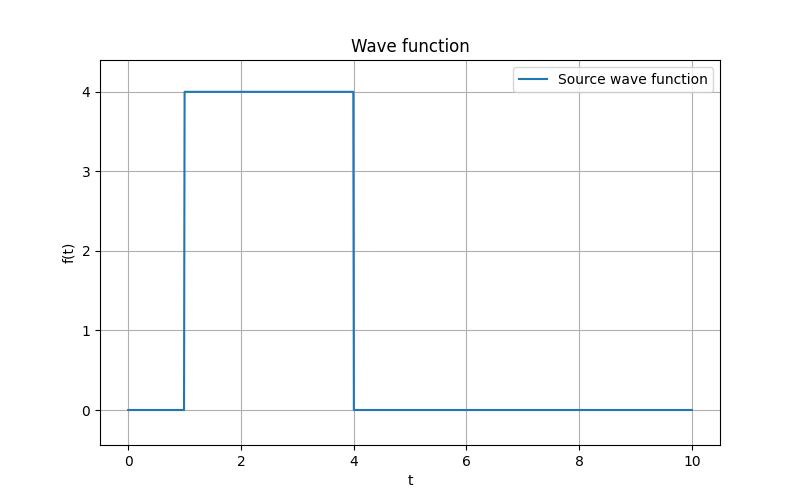
\includegraphics[width=\textwidth]{../results/second/\num/wave_func.png}
    \caption{Функция $g(t)$ с параметрами $a = \a$, $t_1 = \from$, $t_2 = \to$}
    \label{fig:wave_func_\num}
\end{figure}

\begin{figure}[ht!]
    \centering
    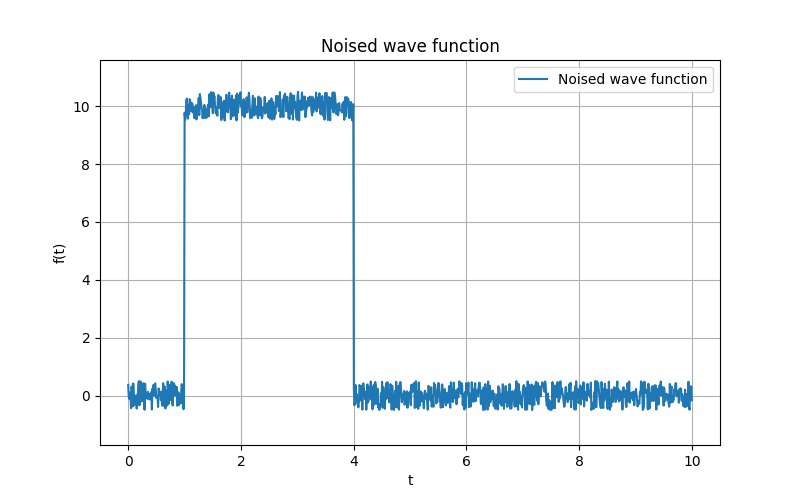
\includegraphics[width=\textwidth]{../results/second/\num/noised_wave_func.png}
    \caption{Функция $u(t)$ с параметрами $b = \b$, $c = \c$, $d = \d$}
    \label{fig:noised_wave_func_\num}
\end{figure}

Рассмотрим фильтрованную функцию $u'(t)$, которая получается применением линейного фильтра второго порядка с $T_1 = \Tf$, $T_2 = \Ts$, $T_3 = \Tt$ (см. рисунок \ref{fig:noised_wave_func_filtered_\num}).
Значения $T_1,~T_2,~T_3$ получены из формул \eqref{eq:t_params} при $w_0 = \Wz$ и $A = \A$.
АЧХ данного фильтра приведена на рисунках \ref{fig:filter_frequency_response_\num} и \ref{fig:filter_frequency_response_log_\num}.

\begin{figure}[ht!]
    \centering
    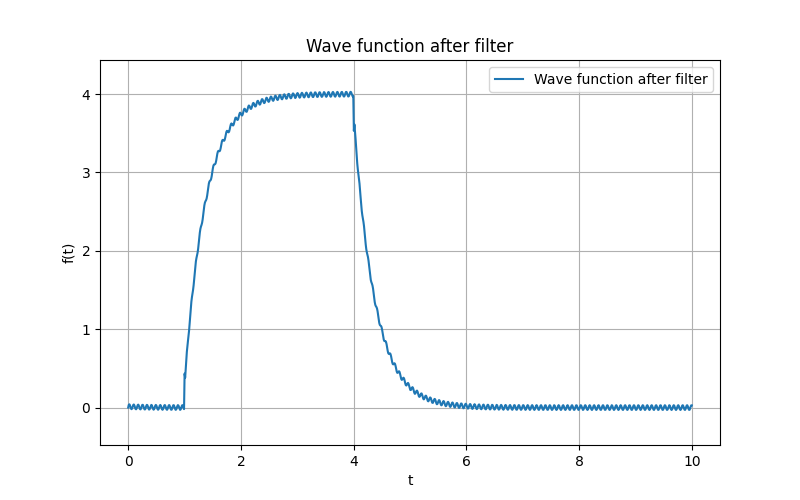
\includegraphics[width=\textwidth]{../results/second/\num/noised_wave_func_filtered.png}
    \caption{Функция $u'(t)$ после применения фильтра}
    \label{fig:noised_wave_func_filtered_\num}
\end{figure}

\begin{figure}[ht!]
    \centering
    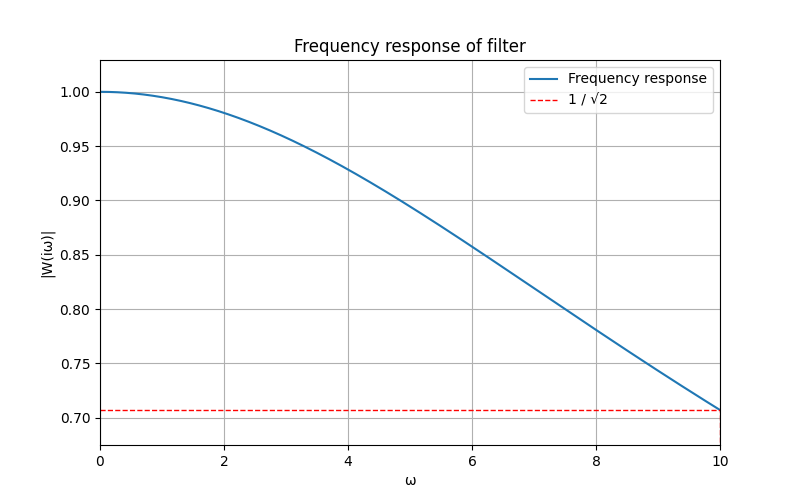
\includegraphics[width=\textwidth]{../results/second/\num/filter_frequency_response.png}
    \caption{АЧХ фильтра второго порядка при $T_1 = \Tf$, $T_2 = \Ts$, $T_3 = \Tt$}
    \label{fig:filter_frequency_response_\num}
\end{figure}

\begin{figure}[ht!]
    \centering
    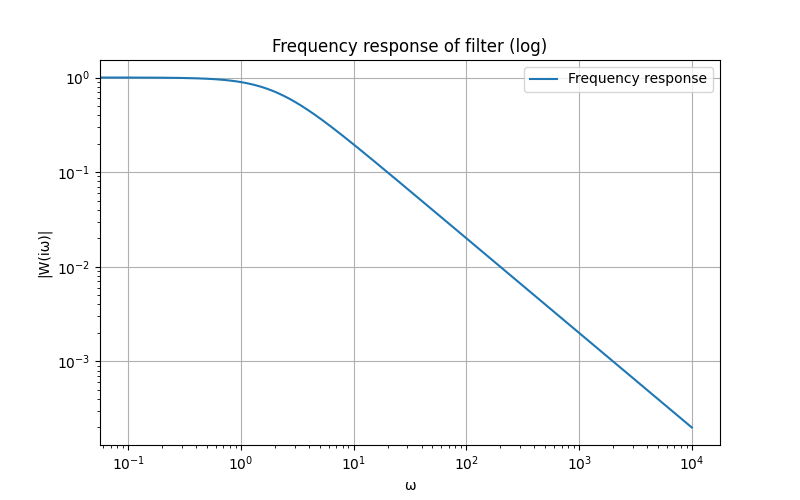
\includegraphics[width=\textwidth]{../results/second/\num/filter_frequency_response_log.png}
    \caption{АЧХ фильтра второго порядка при $T_1 = \Tf$, $T_2 = \Ts$, $T_3 = \Tt$ (логарифмическая шкала)}
    \label{fig:filter_frequency_response_log_\num}
\end{figure}

Видно, что гармонический шум практически полностью был убран, при этом сама функция сохранила свой вид. 
Сравнительные графики исходной и фильтрованной функции приведены на рисунке~\ref{fig:wave_func_cmp_\num}.

\begin{figure}[ht!]
    \centering
    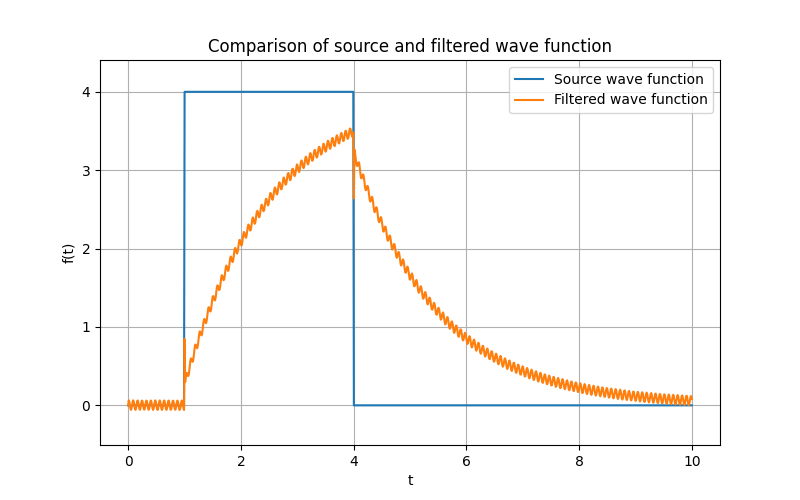
\includegraphics[width=\textwidth]{../results/second/\num/wave_func_cmp.png}
    \caption{Сравнение функции $g(t)$ и $u'(t)$}
    \label{fig:wave_func_cmp_\num}
\end{figure}

\subsubsection{Исследование влияния параметра c на результат фильтрации}


\def\num{8}
\def\a{4}
\def\from{1}
\def\to{4}
\def\b{0}
\def\c{2}
\def\d{80}
\def\L{10}
\def\A{30}
\def\Wz{80}
\def\Tf{\fpeval{round(1 / \Wz, 7)}}
\def\Ts{\fpeval{round(\A / \Wz, 7)}}
\def\Tt{\fpeval{round(1 / (\A * \Wz), 7)}}

Рассмотрим функцию $g(t)$ при параметрах $a=\a$, $t_1 = \from$, $t_2 = \to$ ~(см. рисунок~\ref{fig:wave_func_\num}) 
и ее \textit{зашумленную} версию $u(t)$ с параметрами $b = \b$, $c = \c$, $d = \d$ ~(см. рисунок~\ref{fig:noised_wave_func_\num}).
на промежутке $[0,\L]$. 

\begin{figure}[ht!]
    \centering
    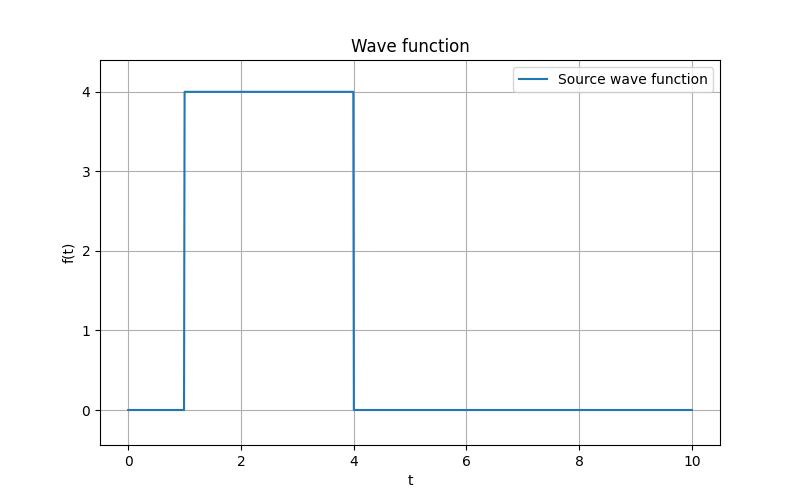
\includegraphics[width=\textwidth]{../results/second/\num/wave_func.png}
    \caption{Функция $g(t)$ с параметрами $a = \a$, $t_1 = \from$, $t_2 = \to$}
    \label{fig:wave_func_\num}
\end{figure}

\begin{figure}[ht!]
    \centering
    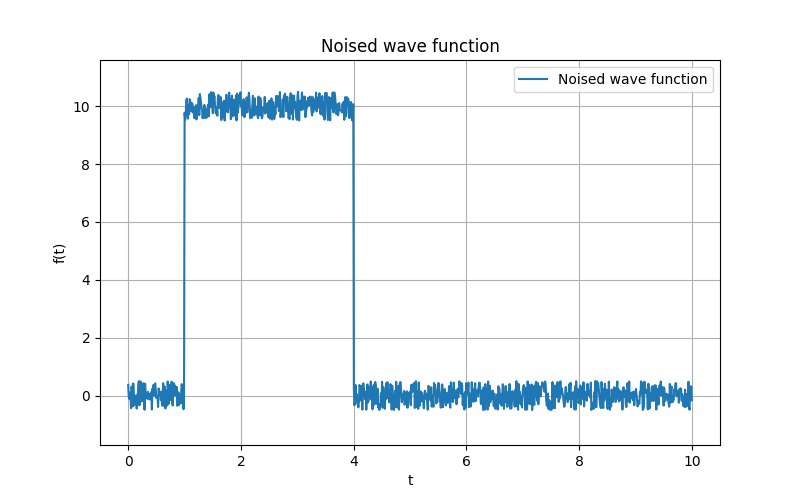
\includegraphics[width=\textwidth]{../results/second/\num/noised_wave_func.png}
    \caption{Функция $u(t)$ с параметрами $b = \b$, $c = \c$, $d = \d$}
    \label{fig:noised_wave_func_\num}
\end{figure}

Рассмотрим фильтрованную функцию $u'(t)$, которая получается применением линейного фильтра второго порядка с $T_1 = \Tf$, $T_2 = \Ts$, $T_3 = \Tt$ (см. рисунок \ref{fig:noised_wave_func_filtered_\num}).
Значения $T_1,~T_2,~T_3$ получены из формул \eqref{eq:t_params} при $w_0 = \Wz$ и $A = \A$.

\begin{figure}[ht!]
    \centering
    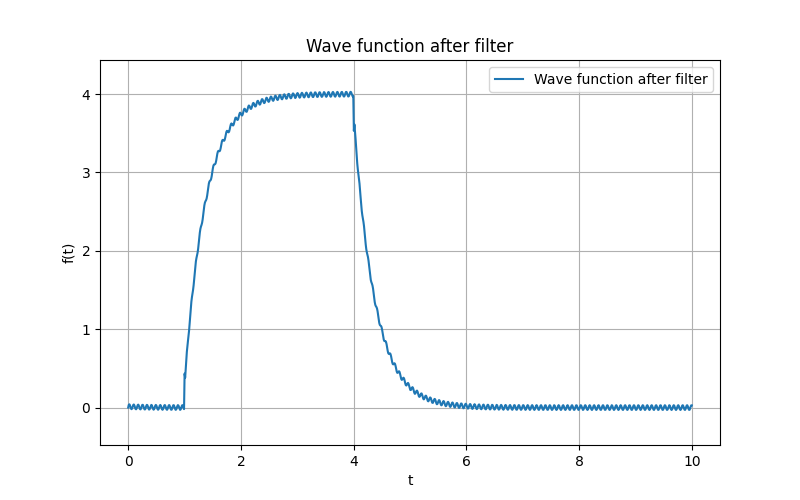
\includegraphics[width=\textwidth]{../results/second/\num/noised_wave_func_filtered.png}
    \caption{Функция $u'(t)$ после применения фильтра}
    \label{fig:noised_wave_func_filtered_\num}
\end{figure}

Сравнительный график исходной функции и функции после фильтрации представлен на рисунке \ref{fig:wave_func_cmp_\num}.

\begin{figure}[ht!]
    \centering
    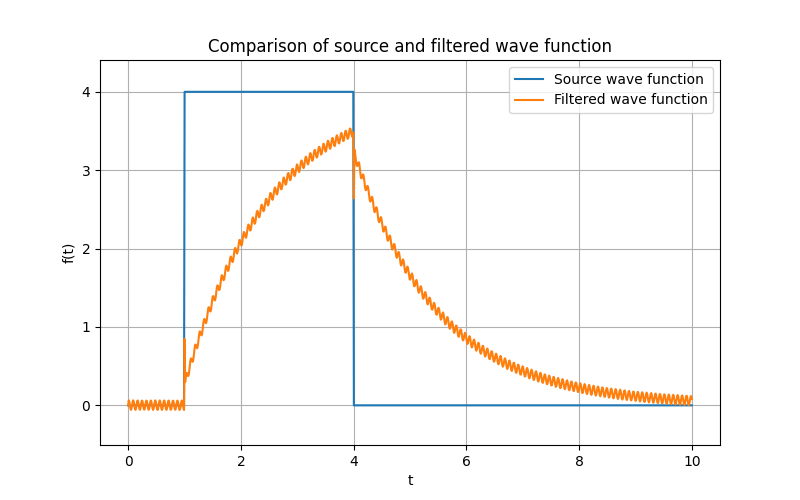
\includegraphics[width=\textwidth]{../results/second/\num/wave_func_cmp.png}
    \caption{Сравнение функции $g(t)$ и $u'(t)$}
    \label{fig:wave_func_cmp_\num}
\end{figure}

Видно, что, как и в первом случае, гармонический шум был успешно убран, несмотря на то, 
что его амплитуда довольно сильно увеличилась (более, чем в 4 раза). Это связано с тем, что 
фильтр подавляет частоты, на которых находится гармонический шум, при этом шум любой амплитуды
будет подавляться пропорционально. 